% Pic of the tiny motor and few other parts

\chapter{Size and weight}
The size and weight of the robot is one of the critical design considerations, It is essential to look at it in more details, to better understand what limits the size of the robot, and what is potentially its smallest size. Our focus is a fully functional robot that includes: microcontroller, wireless communications, actuators, and a battery. 

\section{Sizes of similar robots}
To understand the size limitations of robots, its worth to look at other small robots, even if they don’t employ vertical climbing. In robotics literature, the definition of “small” has been used very loosely, as it is relative to the type of devices. %A one way is to use a convention where \textit{microrobot} is less than 1mm. Mini robot is 

\textbf{Mini robot.}
Using conventional fabrication techniques and off the shelf parts, the smallest size of an untethered robot is about 2 cm. For example, TinyTerp is 2.0 cm~\cite{sabelhaus2013tinyterp} , ALICE is also 2.0 cm and 30 grams~\cite{caprari2001fascination}, and Kilobot is 3.3 cm and 16 grams~\cite{rubenstein2012kilobot}. All of those robots contain microcontroller, radio and employ DC motors, to move on the flat horizontal surface. They are mostly designed for studying swarm behaviors. 

\textbf{Micro robot.}
With microfabrication techniques, the size of the robot can be further reduced. For example, recently microfabricated robots were 0.4cm~\cite{iwata2016insect}.  and a solar-panel powered 0.39 cm robot~\cite{edqvist2009evaluation}. At sub centimeter scales DC motors become impractical; therefore, other actuator mechanisms such as piezoelectricity are used.

\textbf{Sub-millimeter robots.}
Furthermore, using biological and molecular engineering nano-sized robots were created. For example, optical tweezers use a laser to move nanoparticles~\cite{curtis2002dynamic} or catalytic reaction can be used to move nanomotor~\cite{paxton2004catalytic}. Also, the magnetic field could be used to force magnetotactic bacteria to move objects~\cite{martel2006controlled}.

\section{Individual parts size}
It is useful to estimate the smallest potential size of an untethered robot using off-the-shelf parts. Potentially, homebrew parts can be smaller but would require significant research. 

\textbf{Electronics.}
Due to the constant miniaturization electronics are not the limiting size and weight part. It is possible to get a microcontroller with the size of 7x7x0.85 mm (NRF52832, Nordic), that contains a radio, as well as many peripheral interfaces. With a few passive parts and motor drives, it is enough for a self-contained robot. 

\textbf{Batteries.}
Batteries are one of the hardest components to initialize. Motors and actuators have a large instantaneous current draw, therefore require ample discharge rate. Currently, there is only one technology that can practically work in miniature robots: lithium polymer (Li-Po) batteries. Such batteries have high discharge current, small size, high energy density, and can be recharged. Some of the most miniature Li-Po cells have dimensions of 3x9x10 mm (GM300910H, PowerStream) and weight of 0.33grams. The capacity of such a battery is 12mAh and maximum discharge current of 6mAh.  

There are exotic smaller energy sources, such as supercapacitors. Such energy sources are ill-suited for self-powered robots as they do not contain enough energy to power the robot continuously for a few hours. Using such energy sources would require energy harvesting.

\textbf{Actuators.}
Robotics requires large torques; therefore, the motors need to have gearboxes (typically planetary). We successfully used 6mm geared brushed DC motors (TGPP06-D-136, TT Motor) in the Rovables project. The smallest motor (03A, Faulhaber) that provided enough torque was 3.4mm in diameter. There are smaller motors such as stepper motors, but such motors are not designed for high torque applications.  The linear motors tend to be larger, as they require a rack-pinion mechanism or ball-screw to convert rotation into linear motion. 

The skin moving robots require solenoids and pumps as well as motors. The current off-the-shelf solenoid and pumps are too large, therefore had to be placed off-the-robot. Miniaturization of such parts is possible but requires custom engineering. The smallest diaphragm pump that we found is about 8x32x18mm in size and weights x grams (SC3101PM, Skookum Electronic co.). This pump is designed for medical device applications such as miniature arm cuff for blood pressure. Potentially, diaphragm pumps can be smaller by reducing the size of the piston. Figure~\ref{fig:pumps} shows the dimensions of different components and piezoelectric pumps.  

\begin{figure}[!ht]
\centering
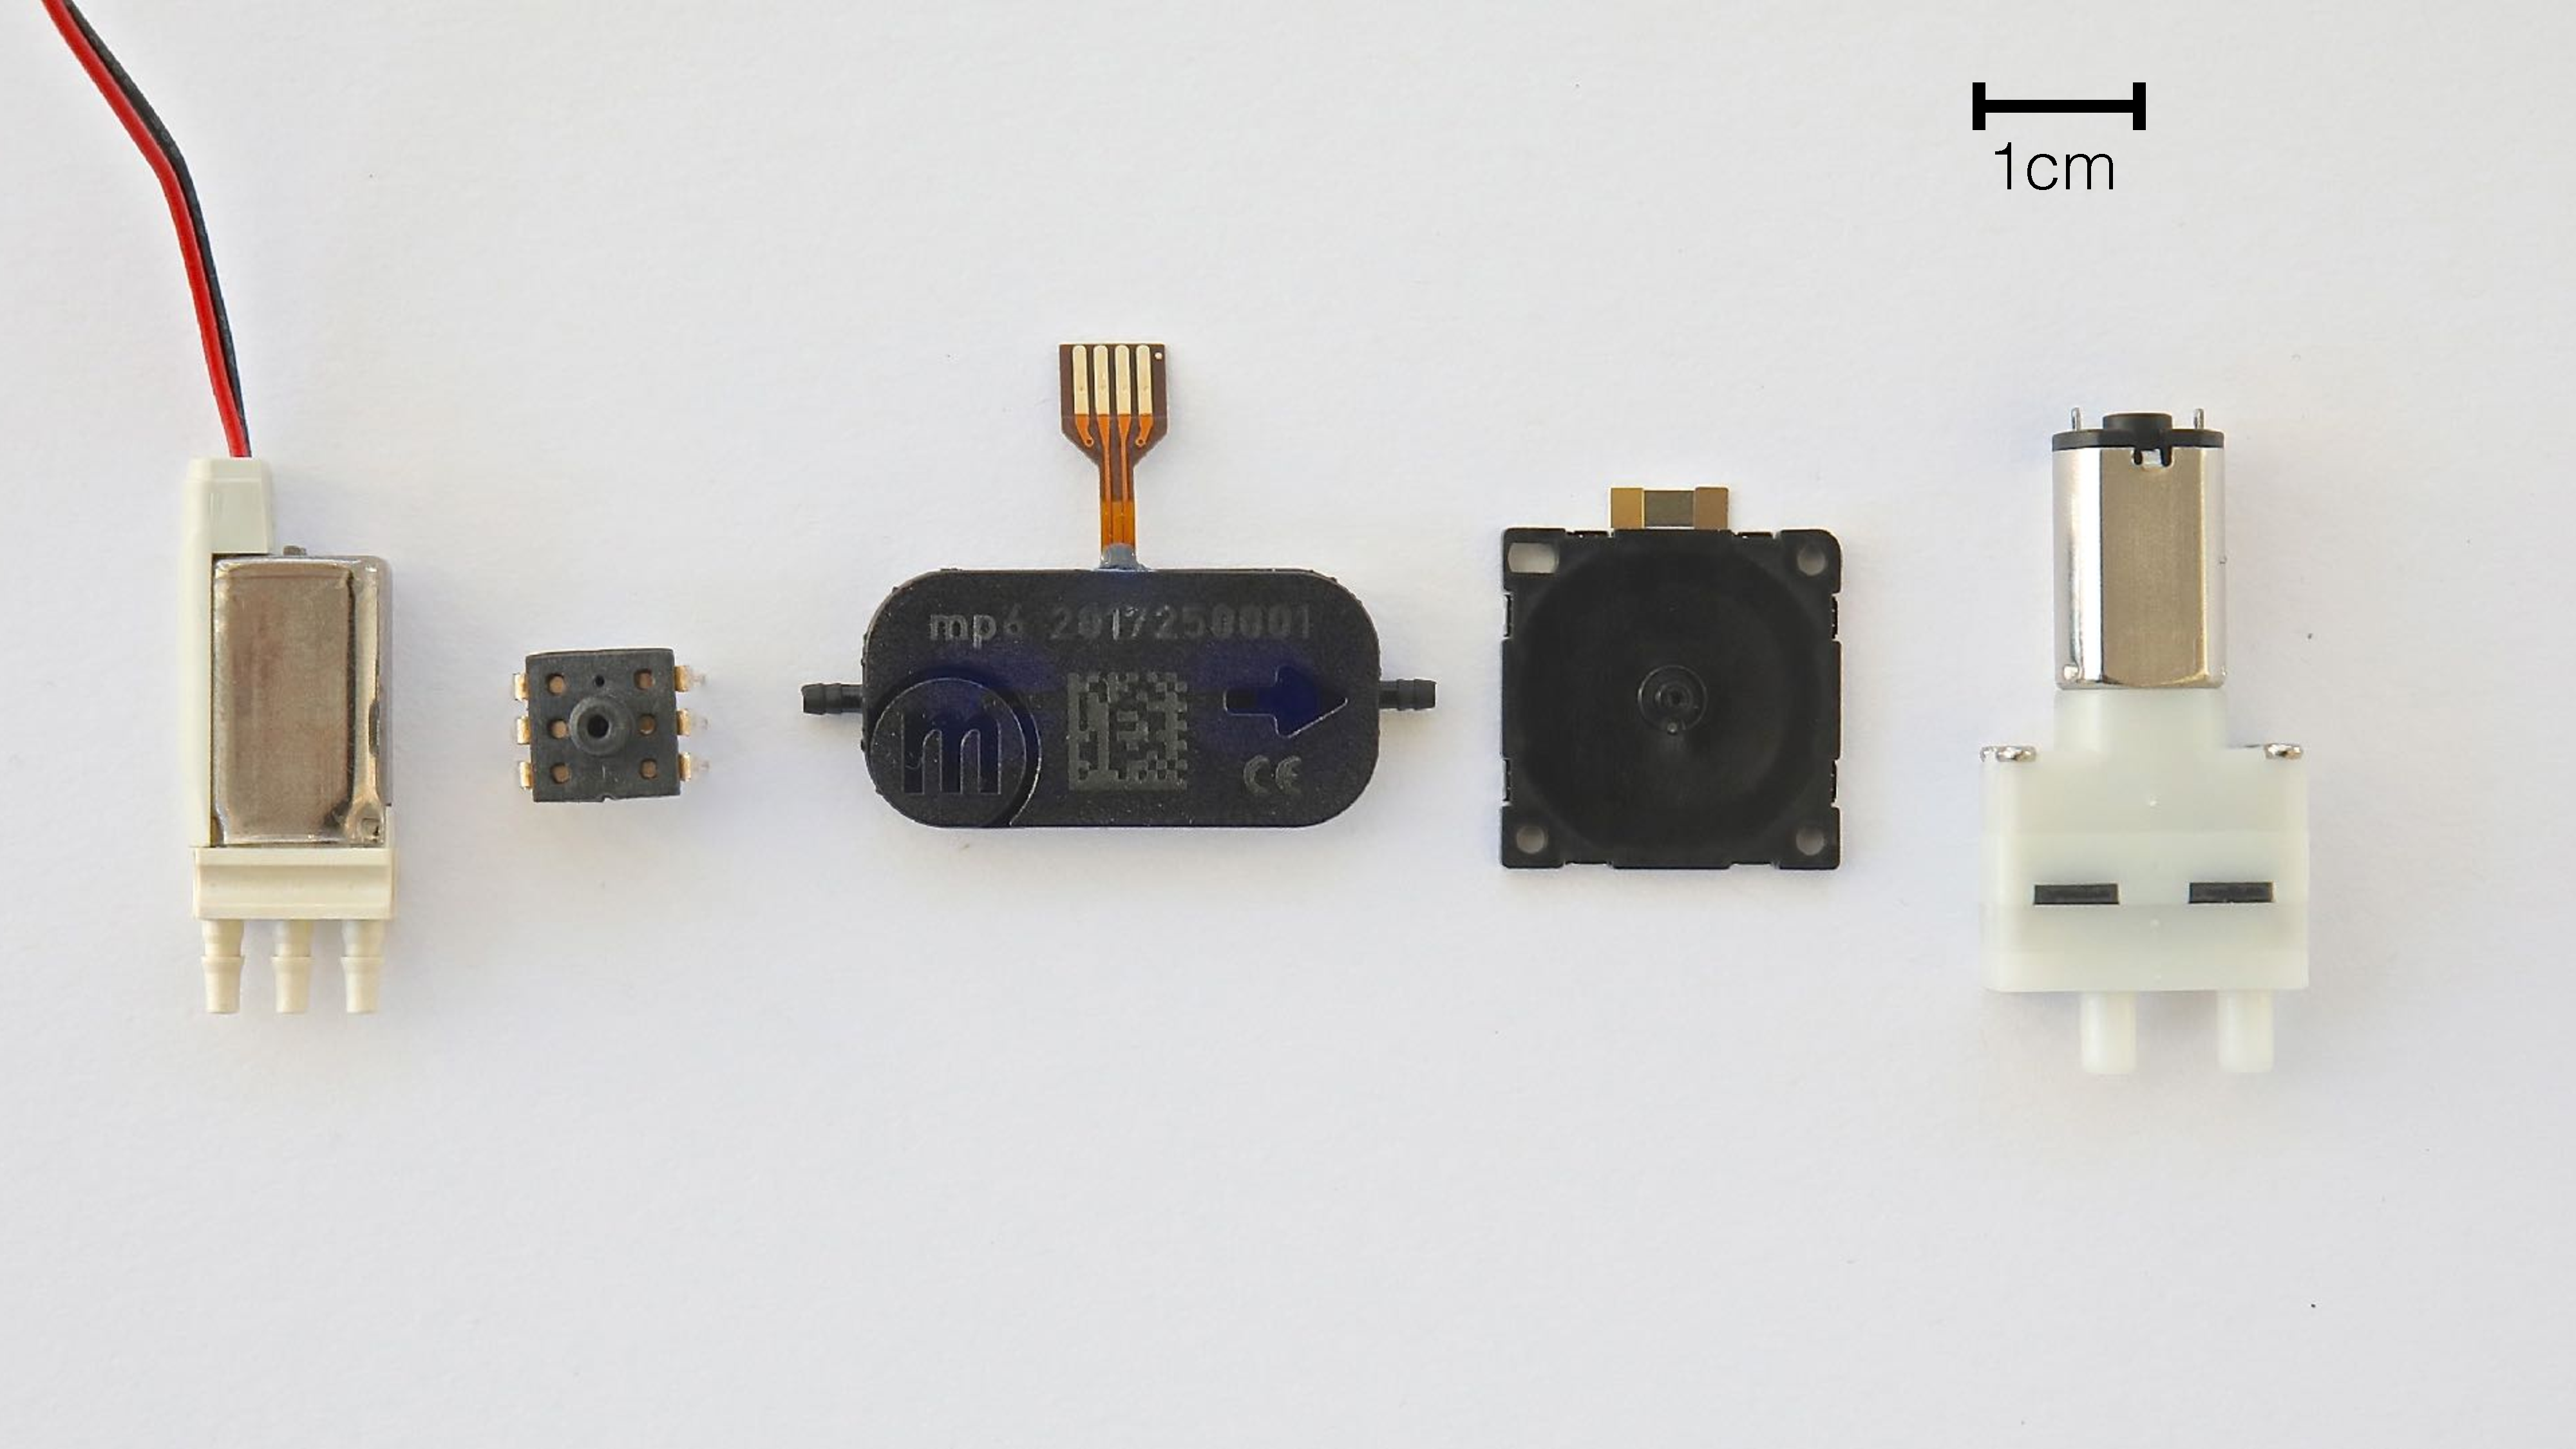
\includegraphics[width=14.0cm]{pictures/chapter6/different_pumps_sizes.pdf}
\caption{Comparison of different compoments sizes that can be used for pneumatics in epidermal robots. Left to right: solenoid, pressure sensor, piezoelectric pump, piezoelectric blower, diaphram pump with DC motor. }
\label{fig:pumps}
\end{figure}

\textbf{Mechanical.}
With the state-of-the-art  3D printing, the minimum resolution is about 25-100 um. With injection molding or CNC, machining resolution can be reduced to 20 um or less. Also, the materials require about 1mm thickness to provide enough structural rigidity. Also, the thickness of FR-4, which is used for the printed circuit boards, should be above 0.5mm to provide enough structural rigidity. The flexible electronics technology allows circuits with a thickness of 0.15mm, so it is an attractive option for miniaturization if no structural rigidity is needed. 

\textbf{Sensors.}
The robot requires to have sensors, which add to the size and weight. Fortunately, sensors are small in comparison to other parts, as they do not need to contain moving parts. Mainly, the robot requires inertial and optical sensors. The inertial sensing can be done using a solid-state inertial measurement chip with the size of 4x4x0.9mm (MPU6050, Invensense). The optical encoders can be the size of a small surface mount LEDs. The camera is larger, as it requires imaging chip, auxiliary components, and a lens. The camera that we use has to die dimensions of  5x5 mm (OV6920, OmniVision). It provides 5 Megapixel resolution, which is enough for machine vision. Additional processing power and memory might be required to do real-time machine vision on-board. 
%https://drum.lib.umd.edu/bitstream/handle/1903/15587/TR_2014-07.pdf?sequence=4&isAllowed=y
\begin{figure}[!ht]
\centering
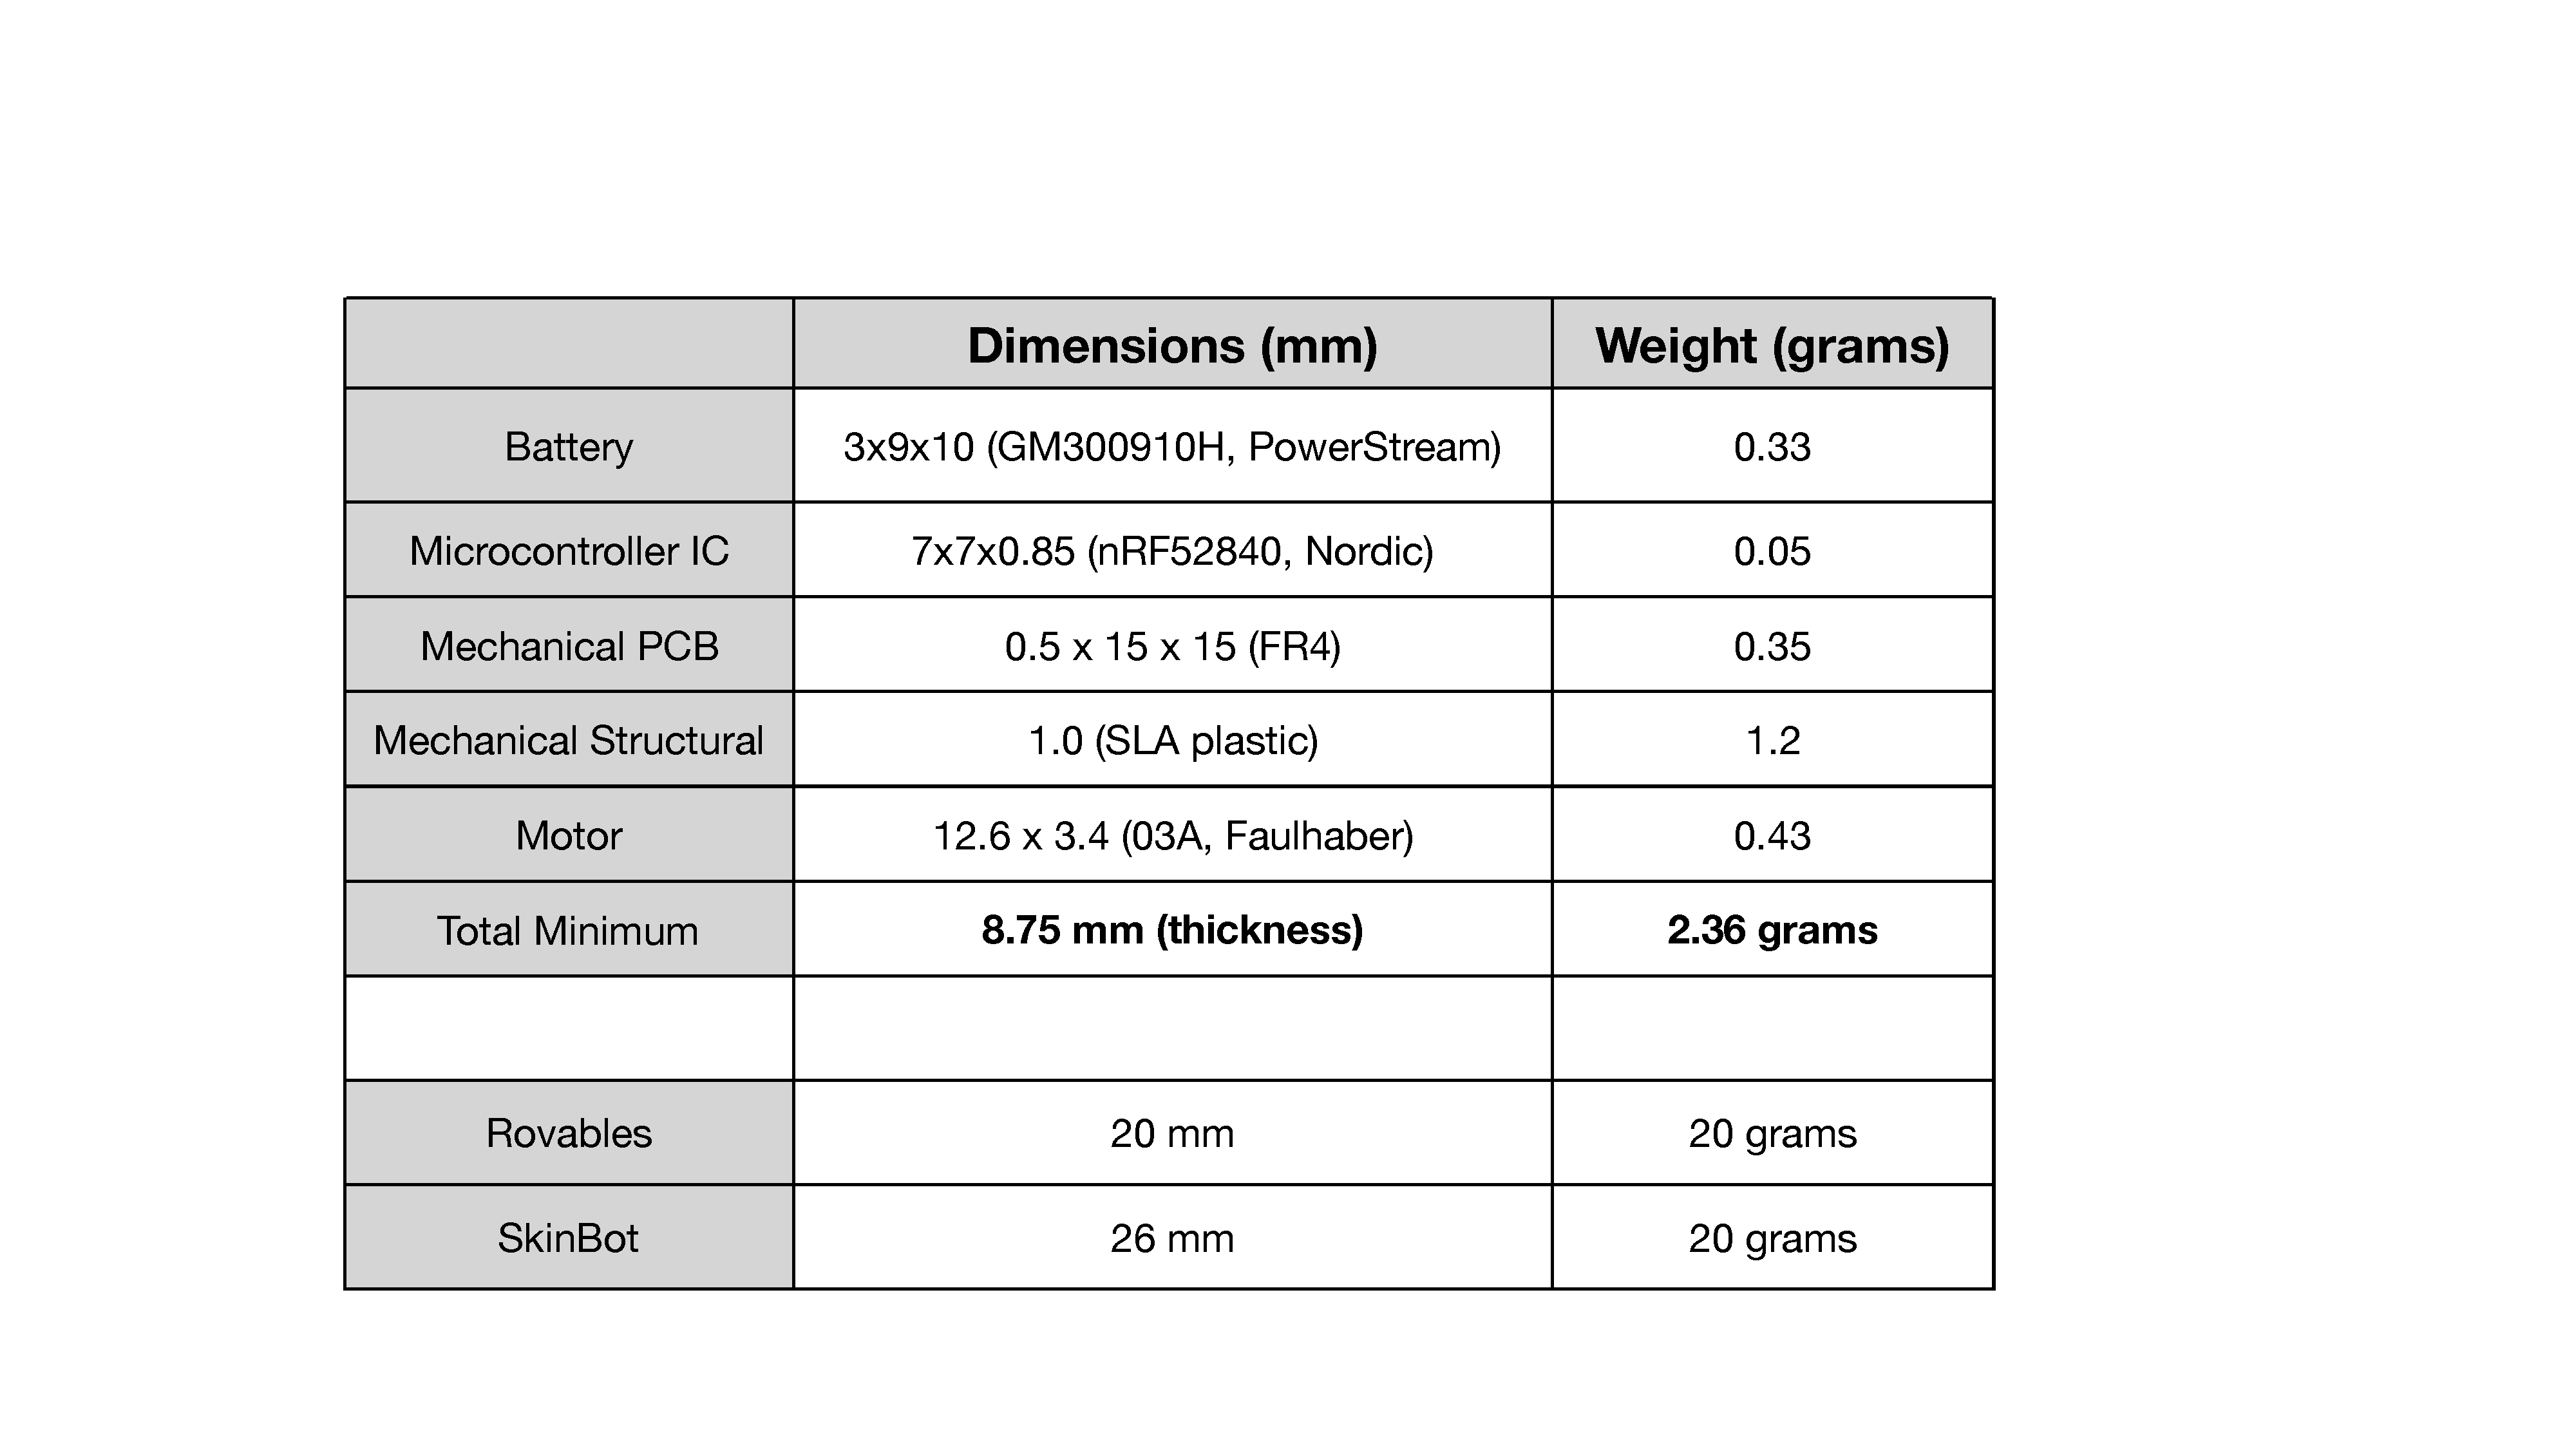
\includegraphics[width=14.0cm]{pictures/chapter6/pic_comparison_sizes_robots.pdf}
\caption{Table showing minimum sizes and weights of different components. Size and weight of Rovables and SkinBot is shown for comparison }
\label{fig:size_weight_min}
\end{figure}

\section{Summary}
It appears that the minimum size and weight of a fully functional robot using off-the-shelf parts is at least 8mm thickness and 2.4 grams. This data is summarized in Figure~\ref{fig:size_weight_min} This number is further confirmed by looking at other miniature research robots, which achieved a size of 2 cm. State-of-the-art electronics and sensors already fit well under the centimeter. On the other hand, most batteries and actuators are well above centimeter in size. The size can be further reduced but requires novel and custom parts that are specifically designed for the application. With the current size of 2cm and weight of 20 grams, DWT robots could be further miniaturized using off-the-shelf parts and extensive engineering. 



